\documentclass[letter, 11pt]{article}
\usepackage[utf8]{inputenc}
\usepackage[spanish]{babel}
\usepackage{amsfonts}
\usepackage{longtable}
\usepackage{amsmath}
\usepackage[dvips]{graphicx}
\usepackage{url}
\usepackage{hyperref}
\usepackage[top=3cm,bottom=3cm,left=3.5cm,right=3.5cm,footskip=1.5cm,headheight=1.5cm,headsep=.5cm,textheight=3cm]{geometry}
\usepackage{listings}
\usepackage{color}
\usepackage{fancyvrb}
\usepackage{fancyhdr}
\usepackage{setspace}
\usepackage{fmtcount}
\usepackage{slashbox}
\renewcommand{\rmdefault}{phv} % Arial
\renewcommand{\sfdefault}{phv} % Arial

\definecolor{red}{rgb}{1,0,0}
\definecolor{green}{rgb}{0,1,0}
\definecolor{blue}{rgb}{0,0,1}
\newcommand{\blue}{\textcolor{blue}}
\newcommand{\red}{\textcolor{red}}
\newcommand{\green}{\textcolor{green}}


%%%%%%%%%%%%%%%%%%%%%%
%Estilo del documento%
%%%%%%%%%%%%%%%%%%%%%%
\pagestyle{fancy}
\onehalfspacing

%%%%%%%%%%%%%%%%%%%%%%%%%%%%%%%%%%%%%%%%%%%
%Fancyheadings. Top y Bottom del documento%
%%%%%%%%%%%%%%%%%%%%%%%%%%%%%%%%%%%%%%%%%%%
% Recuerde que en este documento la portada del documento no posee
% numeracion, pero de igual manera llamaremos a esa primera pagina la numero
% 1, y la que viene la dos. Esto es para tener una idea de las que
% llamaremos pares e impares
\lhead{Tercer Informe} %Parte superior i\include{quierda}
%\rhead{\bf \it Primer Informe} %Parte superior derecha
\lfoot{Universidad Técnica Federico Santa María} %Parte inferior i\include{quierda.}
\cfoot{} %Parte inferior central
\rfoot{\bf \thepage} %Parte inferior derecha
\renewcommand{\footrulewidth}{0.4pt} %Linea de separacion inferior

\begin{document}
\renewcommand{\tablename}{Tabla}

\renewcommand{\listtablename}{Índice de tablas}

\begin{titlepage}
    \begin{center}
	\begin{tabular}{c}
		
\includegraphics[width=0.4\textwidth]{img/utfsm}
	    \vspace{4cm}
	\end{tabular}
	\vspace{6cm}
	\begin{tabular}{c}
		\huge{\sc{Trabajo Recuperativo}}\\\\
		\large{\sc{Evaluación de Proyectos}}
	\end{tabular}
    \vspace{1cm}
	\begin{tabular}{rcl}
			Nombre del Profesor & : & Johana Moya Alfaro\\
			Nombre del Ayudante & : & Teresa Paez\\
								& : & Melissa Ruiz\\
			Datos del Alumno    & : & Cristián Maureira\\
                                & : & 2673030-9
	\end{tabular}

    \vspace{1cm}

    \normalsize{\sc{\today}}\\

	\end{center}
\end{titlepage}


\tableofcontents
\listoffigures
\listoftables

\section{Resumen Ejecutivo}

En el presente informe se detallarán distintos ámbitos del proyecto \emph{Music Labs},
en la sección de Análisis organizacional se especifica que será una estructura
vertical debido al grado de complejidad de la empresa, empezando por los dueños,
un nivel posterior el administrador y secretaría, y en último nivel las unidades
de informática, gestión de eventos, finanzas y sonido, que estarán en el mismo
nivel de toma de decisión.

Por otro lado \emph{Music Labs} se guiará rigurosamente por el Código del Trabajo,
el Artículo 7 para la redacción y contenido de los contratos.
Por consiguiente si se da término al contrato se utilizará el artículo 159 que
enumera los distintos motivos posibles, excluyendo el término del contrato por
necesidad de la empresa el cuál es detallado en el artículo 161.

Los trabajadores además recibirán constante capacitación de acuerdo a los artículos
180 al 183.
Las remuneraciones de los trabajadores han sido establecidas mediante
la complejidad del trabajo, el cargo de trabajo y el título del trabajador.

La sección del Marco legal especifica la legislación actual por la que se regirá
\emph{Music Labs} para cumplir a cabalidad con la Leyes Chilenas.
La Jornada de trabajo no excederá las 48 horas semanales (Artículo 22, Código
del Trabajo) y 1 hora para almuerzo, además de las horas extraordinarias como
se detalla en el Código del Trabajo.

Existirán dos tipos de trabajadores: los Full-time a quienes se le pagará mensualmente y su
sueldo será superior al ingreso mínimo mensual, y los Part-time que se les pagará por cada
hora trabajada.
Además cada trabajador deberá acceder a un seguro obligatorio contra
accidentes de trabajo y enfermedades profesionales, así mismo los trabajadores deberán
estar afiliados a una Isapre o Fonasa, descontando los porcentajes correspondientes del
salario imponible del trabajador (Ley 16.744).

Por otro lado, de acuerdo al D.S. 745 el lugar de trabajo deberá cumplir con las
condiciones básicas sanitarias y ambientales detallando condiciones físicas,
de agua potable y servicios higiénicos.

La seguridad también se detalla mediante el Artículo 40 enumerando las condiciones y cantidad
necesarias de extintores disponibles en el lugar de trabajo y el nivel de ruido al cual serán
expuestos los trabajadores (Artículo 64 al 72).
En esta sección además se detalla de la patente comercial que deberá adquirir la empresa en
la municipalidad de Viña del Mar.
Y por último en esta sección, \emph{Music Labs} cumplirá rigurosamente la Ley del consumidor
detallando los servicios contratados, precios y condiciones de contratación, y que además
la publicidad será verídica en cuanto al servicio, precio y garantía.

La sección correspondiente al estudio tributario da a conocer la fiscalización a la cual
se debe someter la empresa por parte del Servicio de Impuestos Internos (SII),
que involucra el Impuesto al Valor Agregado (I.V.A) que fija una tasa del 19\% a la Sala de Ensayo,
Salón de Eventos, Sala Grabación y Página Web; y el Impuesto a la Renta que fija una tasa del 17\%
de las utilidades del período anual correspondiente.

En la sección Estudio Societario se describe \emph{Music Labs} será una Sociedad por Acciones (SpA)
en donde su objetivo es siempre mercantil, dividiendo su capital en acciones y los accionistas
responden hasta el monto de sus respectivos aportes.
Este tipo de sociedad rescata lo mejor de la Sociedad Responsabilidad Limitada y Sociedad Anónima.
Además se detallan en esta sección los pasos que se deben seguir para formar la sociedad y los costos
que esto conlleva.

La sección siguiente contiene lo referente al Estudio Ambiental, en donde el punto principal es
respecto al ruido (Artículo 146) debido a que el lugar físico de \emph{Music Labs} está dentro de la zona
I (tipo residencial), en donde existe un máximo de ruidos que se deberá emitir. Cabe recalcar que debido
 al rubro de la empresa, ésta no será sometida al Sistema de Evaluación
de Impacto Ambiental descrito en la Ley 19.300.

Finalmente en la sección referente a otros estudios que sean atingentes al proyecto, se explica por qué
no es necesario realizar estudios adicionales.

\section{Conclusiones y Recomendaciones}
La estructura organizacional elegida (horizontal) es la que más se acerca a las 
necesidades de \emph{Music Labs}, debido a la cantidad de gente que se espera esté
trabajando en la organización, además del nivel y rapidez de respuesta que se 
requiere en una empresa como ésta. Por otro lado, es necesario mencionar que 
a pesar de tener cargos específicos, no existe un impedimento real (además del 
trabajo extra) para que una misma persona se haga cargo de más de un área.\\

Para la constitución legal de la empresa, se concluye que las Sociedades por
Acciones son las que presentan una mejor relación costo-beneficio para la misma,
permitiendo establecer libremente una administración propia y con cada
accionista respondiendo hasta el monto de sus respectivos aportes realizados,
entre otros beneficios.\\

En el aspecto legal es fundamental que el proyecto esté sujeto, en todas las
etapas de vida, a la legislación vigente. Esto es importante por varias 
razones, en primer lugar al cumplir con el marco legal en cuanto a las condiciones
entregadas a los trabajadores se lograrán mejores resultados en el trabajo
realizado, ya que estudios han demostrado que el trabajador tiene mejor rendimiento
cuando siente estabilidad, seguridad y justicia en las condiciones en que trabaja.
En segundo lugar, es importante contar con las medidas de seguridad necesarias para
prevenir accidentes y para proteger a los trabajadores de enfermedades laborales, 
en el caso de este proyecto una de las fuentes de enfermedad es la constante
exposición a presión sonora elevada. Esto es importante por la salud de los
trabajadores y para evitar la aplicación de multas y/o sanciones.
Respecto a la ley del consumidor es importante considerarla en todos los procesos, ya 
que servirá de base para lograr entregar un servicio de calidad y del gusto del cliente, 
y por supuesto cumplir con las leyes y evitar multas.\\

Considerando el estudio tributario, se puede notar de que no existen impuestos
adicionales que pudiesen perjudicar el presente proyecto, puesto que sólo
es necesario tomar en cuenta el Impuesto al Valor Agregado por los servicios
que se ofrecerán e Impuestos a la Renta para las personas que trabajarán
dentro de \emph{Music Labs}. 

\subsection*{Recomendaciones}
Se recomienda contar con asesoría legal periódica que permita mantener
al proyecto actualizado en cuanto a las leyes que le afectan para prevenir
multas o problemas judiciales por el no cumplimiento. Una vez obtenida la
patente comercial es importante que año a año se vaya entregando la
documentación necesaria para la renovación de ésta.


\section{Análisis Organizacional}
%MARITO

\subsection{Estructura Organizacional}
%MARITO

La estructura organizacional que utilizará \emph{Music Labs}
será la horizontal, pues debido al tamaño de la empresa no tiene 
sentido realizar una gran verticalidad en los cargos. Además, en este 
tipo de empresas, se requiere respuestas rápidas, y buen contacto
de la ``plana mayor'' con todos los trabajadores, lo cual se complica 
teniendo una estructura vertical, debido a la burocracia que puede 
existir al momento de tomar una decisión importante. Esta estructura básicamente
consiste en mantener un administrador de tiempo completo, junto a su secretario(a), 
que será quien tiene a cargo la empresa. Sobre él recaerá cada una de las unidades 
de la organización, que se dedican a un área específica. 
\begin{figure}[h!t]
   \centering
  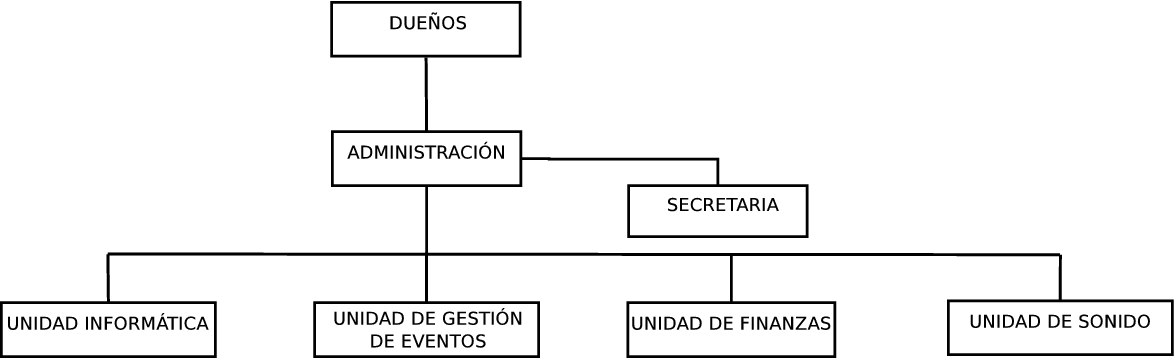
\includegraphics[scale=0.4]{img/estructuraorganizacional.png}
   \caption{Estructura organizacional}
   \label{fig:Estructura organizacional}
\end{figure}

A continuación se detallan cada una de las áreas de la estructura
organizacional:

\begin{itemize}

	\item Dueños: Corresponden a las personas dueñas del negocio en sí. Pueden (o no)
	permanecer en el lugar en que la organización se desempeña. Son los dueños del capital
	inicial, y a quienes deben rendirle cuentas cada una de las unidades de la empresa.

	\item Administrador: De preferencia, este cargo debe recaer en un
	 Ingeniero Industrial, Comercial, de Proyectos, o similar. Su función principal
	consiste en la coordinación de las 4 unidades que se encuentran bajo su cargo. Además, debe 
	velar por el buen funcionamiento de la empresa, y entregar reportes relevantes a los dueños, 
	en caso de ser requeridos. 
	
	\item Secretario(a): Entregar el apoyo que sea necesario al administrador. Además, todas 
	las solicitudes de sala de ensayo, estudio de grabación, entre otras, serán gestionadas por él.

	\item Encargado Unidad Informática: De preferencia, este cargo debe recaer en un 
	Ingeniero Informático o similar. Su función principal es la de encargarse de los clientes
	que solicitan el apoyo de posicionamiento en la web 2.0. En caso de verse sobrepasado por 
	las bandas que requieren de este servicio, está facultado para contratar (en base a 
	honorarios) a programadores que puedan realizar el trabajo, previo aviso al administrador.

	\item Encargado Unidad de Finanzas: De preferencia, este cargo debe recaer en un Ingeniero
	Comercial, o en un Contador. Su función principal consiste en estar al tanto de todos los 
	movimientos financieros que se realicen dentro de la empresa, además de la declaración de 
	los impuestos en el momento en que corresponda. Otra tarea a cumplir, es la de estar
	a cargo de las remuneraciones de las personas que trabajan dentro de \emph{Music Labs}.

	\item Encargado Unidad de Gestión de Eventos: Su función principal es la de canalizar 
	las solicitudes de eventos por parte de las bandas. Estos eventos pueden ser realizados 
	tanto en locales externos, como de \emph{Music Labs}. Esto lleva a definir ciertas subtareas, 
	que son determinar el monto a pagar, cantidad de personas, equipos necesarios, etc.

	\item Encargado Unidad de Sonido: De preferencia, este cargo debe recaer en un Ingeniero 
	en Sonido, o similar. Su función principal es la de encargarse del funcionamiento de la
	sala de ensayo y el estudio de grabación. En particular, debe estar capacitado para poder
	asistir a las bandas al momento que decidan grabar sus discos. 

\end{itemize}

Cabe destacar que cada una de las unidades tiene personas a su cargo, pero estas personas son llamadas
según sea la necesidad de la empresa. No son funcionarios de planta. 

\subsection{Leyes laborales atingentes al proyecto}
%Javier

Para dejar claramente establecido, y en palabras del artículo 3 del Código del Trabajo\footnote{Código del
trabajo del Ministerio de Trabajo y Previsión Social}, se entiende por:

\begin{itemize}
  \item \textbf{Empleador}: la persona natural o jurídica que utiliza los servicios intelectuales o materiales
de una o más personas en virtud de un contrato de trabajo.
  \item \textbf{Trabajador}: toda persona natural que preste servicios personales intelectuales o materiales, bajo
dependencia o subordinación, y en virtud de un contrato de trabajo, y
  \item \textbf{Trabajador Independiente}: aquel que en el ejercicio de la actividad de que se trate no depende de 
empleador alguno ni tiene trabajadores bajo su dependencia.
\end{itemize}

En cuanto al contrato de trabajo la empresa se guiará por lo que dice el artículo 7: \emph{``Contrato individual de trabajo 
es una convención por la cual el empleador y el trabajador se obligan recíprocamente, éste a prestar servicios personales 
bajo dependencia y subordinación del primero, y aquél a pagar por estos servicios una remuneración determinada''}. El 
contrato debe tener, por lo menos, las siguientes estipulaciones:

\begin{enumerate}
  \item lugar y fecha del contrato;
  \item individualización de las partes con indicación de la nacionalidad y fechas de nacimiento e ingreso del trabajador;
  \item determinación de la naturaleza de los servicios y del lugar o ciudad en que hayan de prestarse;
  \item monto, forma y período de pago de la remuneración acordada;
  \item duración y distribución de la jornada de trabajo, salvo que en la empresa existiere el sistema de trabajo por turno, caso en el cual se estará a lo dispuesto en el reglamento interno;
  \item plazo del contrato, y
  \item demás pactos que acordaren las partes.
\end{enumerate}

Respecto al término de contrato de un trabajador estará normado por lo indicado en el artículo
159 del código del trabajo el cual dice que el trabajo terminará en los siguientes casos:

\begin{itemize}
  \item Mutuo acuerdo de las partes.
  \item Renuncia del trabajador, dando aviso a su empleador con treinta días de anticipación, a lo menos.
  \item Muerte del trabajador.
  \item Vencimiento del plazo convenido en el contrato. La duración del contrato de plazo fijo no podrá exceder de un año.
  \item Conclusión del trabajo o servicio que dio origen al contrato.
  \item Caso fortuito o fuerza mayor.
\end{itemize}

Además tal como indica el artículo 161: \emph{``Sin perjuicio de lo señalado en los artículos precedentes, 
el empleador podrá poner término al contrato de trabajo invocando como causal las necesidades de la empresa, 
establecimiento o servicio, tales como las derivadas de la racionalización o modernización de los mismos, bajas 
en la productividad, cambios en las condiciones del mercado o de la economía, que hagan necesaria la separación 
de uno o más trabajadores, y la falta de adecuación laboral o técnica del trabajador''}.\\

En razón de brindar un mejor servicio a los clientes, los trabajadores de la empresa tendrán capacitación
ocupacional acorde al trabajo realizado, siendo una capacitación ocupacional \emph{``el proceso destinado a promover, 
facilitar, fomentar y desarrollar las aptitudes, habilidades o grados de conocimientos de los trabajadores, con el 
fin de permitirles mejores oportunidades y condiciones de vida y de trabajo''}, tal como detalla el artículo 179.
Este tipo de capacitación será entregada en los términos que definen los artículos 180 al 183 del código del
trabajo.\\

Tal como lo estipula el artículo 13 del Código, solamente se contratarán personas mayores de edad, es decir,
personas con 18 años cumplidos o más.\\

Más detalles relacionados con la jornada de trabajo, remuneraciones, seguridad laboral y otros temas laborales están 
detallados en la sección 4 de este informe.

\subsection{Análisis de remuneraciones y sus proyecciones}

A continuación se detallan las remuneraciones que estarán disponibles en cada uno de los cargos
que se describieron anteriormente. Además, se detallará las remuneraciones a honorarios que pueden percibir
las personas que sean contratadas vía necesidad de la empresa.

Cabe destacar que los montos acá nombrados corresponden a la situación en que una persona distinta
esté a cargo de cada unidad nombrada, pero esto eventualmente puede cambiar, pues una misma persona 
perfectamente podría estar a cargo de la Unidad de Eventos y la Unidad de Sonido. En este caso, el sueldo 
final no correspondería a la suma de los 2 cargos, sino que al sueldo de uno de ellos multiplicado por 1.5

\begin{table}[h]
\centering
\begin{tabular}{|c|c|c|c|c|c|c|} \hline
Cargo           & Imponible & AFP      & Salud   & Accidentes & Cesantía & Líquido  \\ \hline
Administrador   & \$1200000 & \$148800 & \$84000 & \$11520    & \$28800  & \$926880 \\ \hline
Unidad Info     & \$1000000 & \$124000 & \$70000 & \$9600     & \$24000  & \$772400 \\ \hline
Unidad Finanzas & \$1000000 & \$124000 & \$70000 & \$9600     & \$24000  & \$772400 \\ \hline
Unidad Eventos  & \$1000000 & \$124000 & \$70000 & \$9600     & \$24000  & \$772400 \\ \hline
Unidas Sonido   & \$1000000 & \$124000 & \$70000 & \$9600     & \$24000  & \$772400 \\ \hline
Secretario(a)   & \$500000  & \$62000  & \$35000 & \$4800     & \$12000  & \$386200 \\ \hline
\end{tabular}
\caption{Sueldos del personal de planta}
\end{table}
En caso de necesitar profesionales o técnicos debido a una gran demanda de funciones (técnicos 
en sonido, programadores, comunicadores audiovisuales, etc), éstos serán trabajadores a honorarios, 
y su paga a recibir corresponderá a \$6000 bruto por hora trabajada, no debiendo exceder las 5 horas diarias de trabajo.

Cada uno de estos sueldos se reajusta de forma anual, en base a los indicadores nacionales más un 2\% sobre el sueldo del año.
Además, los dueños están en su derecho de entregar bonos de desempeño semestrales, en caso de ser necesario.

Si se realiza una proyección a los primeros 5 años en base sólo a sueldos de personal de planta, y sin contar el IPC
nacional, los montos que desembolsará la empresa serán los siguientes:

\begin{table}[h]
\centering
\begin{tabular}{|c|c|c|c|c|c|} \hline
              & Año 1     & Año 2     & Año 3     & Año 4     & Año 5     \\ \hline
Total a pagar & \$5700000 & \$5814000 & \$5930280 & \$6048886 & \$6169863 \\ \hline
\end{tabular}
\caption{Proyección de los sueldos totales a 5 años}
\end{table} 

Estos montos no incluyen al personal que será contratado por necesidad de la empresa, en caso
de que la demanda por parte de las bandas sea mucha. Además, cabe destacar que estos montos corresponden 
al costo Mensual durante el Año X.
\subsection{Tabla resumen de egresos (clasificándolos en inversiones y operacionales)}

La tabla de resumen de egresos corresponde a montos utilizados a lo más dentro del primer año. 
Estos egresos no necesariamente serán replicados en los años posteriores, pues las primeras inversiones
(material musical, instrumentos) no se renuevan año a año.

Para especificar cada uno de los egresos de \emph{Music Labs} se clasificará cada uno de ellos, antes de
mostrar la tabla correspondiente. 

\begin{enumerate}
	\item Costos operacionales
	\begin{enumerate}
		\item Costos Directos: Sueldos.
		\item Costos Indirectos: Si bien no se ha definido aún, el aseo externo puede ser un costo indirecto para la empresa
		\item Costos Fijos: Arriendo.
		\item Costos Variables: Gastos básicos (luz, agua, gas, teléfono)
		\item Gastos Generales: Insumos de oficina.
	\end{enumerate}

	\item Costos de inversión
	\begin{enumerate}
		\item Capital Fijo: Equipos de oficina, sala de ensayo, grabación, sala de eventos, adaptaciones.
		\item Capital Intangible: Costos de formación de sociedad (3.2\% del capital, ver punto 6.3). Suponiendo un capital 
		inicial de 100000000 (cien millones), correspondería a 3200000 (tres millones doscientos mil).
		\item Capital de Trabajo: El capital de trabajo se puede obtener mediante distintos métodos. Se mostrará inicialmente el método de desfase.

		$$
		\frac{\text{número de desfase}*\text{egresos 1º año}}{12}
		$$

		Como se puede apreciar, se toman en cuenta los egresos del primer año, que consideran los sueldos y remuneraciones, entre otras cosas. 
Como esta tabla en general se trata de egresos del primer año, y además, se detallan los costos operacionales por separado, no se considerará el capital de 
trabajo como un ítem separado.
\end{enumerate}
\end{enumerate}
% Arriendo                    & 12000  & 12000  & 12000  & 12000  & 12000  & 12000  & 12000  & 12000  & 12000  & 12000 \\
% Equipos de Oficina          & 655    & 0      & 0      & 0      & 0      & 0      & 367    & 150    & 0      & 0\\
% Equipos Sala de Ensayo      & 6045   & 0      & 0      & 0      & 0      & 0      & 6045   & 0      & 0      & 0 \\
% Equipos Grabación           & 3524   & 0      & 0      & 0      & 0      & 0      & 3524   & 0      & 0      & 0 \\
% Equipos Sala de eventos     & 6000   & 0      & 0      & 0      & 0      & 0      & 6000   & 0      & 0      & 0 \\
% Adaptaciones especializadas & 2616   & 0      & 0      & 0      & 0      & 0      & 0      & 0      & 0      & 0 \\
% Adaptaciones necesarias     & 8719   & 0      & 0      & 0      & 0      & 0      & 0      & 0      & 0      & 0  \\
% Materias primas e insumos   & 92718  & 92718  & 92718  & 92718  & 92718  & 92718  & 92718  & 92718  & 92718  & 92718 \\
% Total anual                 & 132277 & 104718 & 104718 & 104718 & 104718 & 104718 & 120649 & 104868 & 104718 & 104718 \\

%\red{cmaureir:} Estos son los elementos de la tabla de egresos del informe pasado,
%pero no veo como cosas de sueldos y esas cosas, que serían \emph{Costos Directos}
%además hay otros elementos de esta tabla que no tenemos ningún \emph{egreso},
%como lo son:
%\begin{itemize}
%   \item Capital Intangible
%   \item Capital de trabajo
%   \item Costos Indirectos
%   \item Gastos Generales
%   \item Costos Variables
%\end{itemize}
%
%Acá la categorización de los egresos que habíamos puesto en informe 2:
%
%\begin{itemize}
%   \item Arriendo (Costo fijo)                  
%   \item Equipos de Oficina (Capital Fijo)      
%   \item Equipos Sala de Ensayo (Capital Fijo)          
%   \item Equipos Grabación       (Capital Fijo)         
%   \item Equipos Sala de eventos (Capital Fijo)         
%   \item Adaptaciones especializadas (Capital Fijo)      
%   \item Adaptaciones necesarias    (Capital Fijo)      
%   \item Materias primas e insumos (Costos directos) 
%\end{itemize}
%
%\red{cmaureir:} fin comentario (comentado en el .tex están los tipos de elementos de cada punto)

\begin{table}[htb!]
\centering
%\small
\scriptsize
	\begin{tabular}{|l|r|r|}
      \hline
      {\bf Resumen de costos}      & Costo Mensual  & Costo Anual    \\ \hline
      \blue{Costos de Inversión}   &                &                \\ \hline
      Capital Fijo                 & 2297           & 27759          \\ \hline
      Capital Intangible           & -              & -              \\ \hline
      Capital de trabajo           & -              & 3200              \\ \hline
                                   & {\bf Total }   & {\bf 30959 }   \\ \hline
      \blue{Costos Operacionales}  &                &                \\ \hline
      Costos Directos              & 5700           & 68400          \\ \hline
      Costos Indirectos            & No considerado & No considerado \\ \hline
      Gastos generales             & 50             & 600            \\ \hline
      Costos Variables             & 932            & 11182          \\ \hline
      Costos fijos                 & 1000           & 12000          \\ \hline
                                   & {\bf Total }   & {\bf 92182 }   \\ \hline
   \end{tabular}
\caption{Resumen de egresos (en miles)}
\end{table}


%  Capital Fijo:
%     referido al costo de realización física del proyecto y está asociada a inversiones en:
%        -Compra de terrenos
%        -Adquisición de equipos
%        -Construcción de obras civiles
%        -Construcción de proyectos complementatios (alcantarillado, agua potable, tendido eléctrico, líneas telefónicas, etc)
%        -Cañerias, instrumentos, aislamiento.
%  
%  Capital en Intangible:
%     -Costos de ingeniería (asesoramiento técnico y supervisión)
%     -Gastos de administración
%     -Gastos de puesta en marcha
%     -Patentes y licencias
%     -Sistemas de información pre-operativos
%     -Seguros y costo de montaje
%     -Capacitación
%     -Estudios técnicos durante la ejecución
%  
%  Capital de Trabajo
%     Constituye el conjunto de recursos necesarios, en la
%     forma de activos circulantes, para la operación normal del proyecto
%     durante un ciclo productivo, para un tamaño determinado.
%    
%     Métodos de Estimación:
%        -El método contable
%        -El método del periodo de desfase
%        -El método del déficit acumulado máximo
%  
%  Costos Directos:
%     Materias primas y materiales directos
%     Mano de obra directa (incluye supervisión de operación hasta jefe de turno).
%     Comprende sueldos y salarios, gastos previsionales, horas extraordinarias,
%        bonos, incentivos y beneficios adicionales.
%     Insumos directos (energía, combustibles, lubricantes, vapor, agua,
%        refrigeración, etc., cuando corresponda)
%  
%  Costos Indirectos:
%     Mano de obra indirecta (supervisión y mantención general, seguridad
%        industrial, vigilancia, control de calidad, laboratorios, etc.)
%     Materiales Indirectos
%     Otros gastos indirectos (servicio médico, casino, movilización,
%        comunicaciones, iluminación, transporte interno, aseo de planta, etc.)
%     Beneficios del personal (jardín infantil, club de campo, economato, etc.)
%  
%  Gastos Generales:
%     Gastos administrativos (sueldos de personal ejecutivo, comunicaciones e
%        impresiones, aseo de oficinas, útiles de oficina, etc.)
%     Cargos fijos (seguros)
%     Gastos de ventas (sueldos, comisiones, gastos de representación, viáticos,
%        publicidad).
%     Investigación y desarrollo
%     Gastos de financiamiento (intereses y amortización del préstamo)
%  
%  Costos fijos:
%     son independientes del volumen de producción. Ej:
%     depreciación, arriendo, los costos de administración
%  
%  Costos variables:
%     dependen del volumen de producción, pues varían con
%     la producción. Ej: costos de energía eléctrica, de materias primas, ciertas
%     categorías de mano de obra, etc
%  

\section{Estudio Marco Legal}
%[JAVIER]
%[SECCIÓN TERMINADA Y REVISADA ORTOGRAFÍA Y REDACCIÓN]

Es importante verificar, al momento de
evaluar y ejecutar un proyecto, que 
se cumple con la legislación del país.
Para que un proyecto sea factible
debe cumplir a cabalidad con las leyes. 
Para ésto, a continuación, se describirá 
la legislación bajo la cual el proyecto debe 
estar sustentado para poder ser legalmente 
factible, de tal forma de lograr tener
un conocimiento claro al respecto.\\

En primer lugar, parte importante
de toda organización son los
trabajadores. Por esta razón, 
es necesario considerar los 
artículos que el Código del Trabajo
presenta. A continuación se detallan
los principales aspectos del ámbito
del proyecto que se deben considerar.

\subsection*{Jornada de Trabajo}

La jornada de trabajo
no excederá 48 horas semanales
tal como detalla el Artículo 22
del código del trabajo. Ya que
las horas diarias máximas de
trabajo son 10, este será
el límite para la cantidad
de horas normales y extras
de trabajo, según sea necesario.
Las horas extraordinarias estarán
pactadas en el contrato de trabajo
según el artículo 32 del código.
El trabajador contará con 1 hora de
colación, según estipula el 
artículo 34. En cuanto al descanso
semanal estará regulado por el
artículo 35.

\subsection*{Remuneraciones}

La remuneración para el caso de
los trabajadores Full-Time estará
fijada de manera mensual. En cambio,
los trabajadores que sean requeridos
para servicios Part-Time recibirán
remuneración por hora efectiva
de trabajo. El monto mensual
de remuneración será superior
al ingreso mínimo mensual, estando
estipulado en el contrato de trabajo.
En cuanto a la asignación familiar
estará establecida en el contrato.

\subsection*{Ley Número 16.744}
Esta ley establece normas sobre accidentes
del trabajo y enfermedades profesionales.
En primer lugar hay que destacar que todos
los trabajadores contarán con el Seguro
Social obligatorio contra riesgos de Accidentes
del Trabajo y Enfermedades profesionales, según
estipula el artículo 1 y 2 de la ley. Cualquier
situación que ocurra en el trabajo o en el camino
hacia él, será considerada accidente según lo que dicta 
el artículo 5. Las enfermedades profesionales
estarán regidas bajo las indicaciones del artículo 6 y 7.
Las cotizaciones de salud serán realizadas por
la empresa según los términos que establece la Ley
en los artículos 17 y 18. El trabajador deberá
estar afiliado a una Isapre o Fonasa según estime
conveniente. La imposición mensual en una AFP estará
dada según el porcentaje que estipula la ley, descontándose
del salario imponible del trabajador, de manera similar
a la cotización de salud.

\subsection*{Decreto Supremo 745}
Este decreto establece las condiciones sanitarias y 
ambientales básicas que deberá cumplir todo lugar de
trabajo.\\ %Además establece los límites permisibles de 
%exposición ambiental a agentes químicos y agentes físicos, y
%aquellos límites de tolerancia biológica para trabajadores
%expuestos a riesgo ocupacional.


Las condiciones físicas del lugar de trabajo cumplirán
con la especificación entregada en los artículos 4 al 9.
Los servicios básicos como son el agua potable estarán
normados por los artículos 11, 12, 13. Los servicios
higiénicos deben contar con las condiciones mínimas
que estipula el artículo 20, 21, 22, 24. Es decir, serán
baños separados para hombre y mujer, con el número de 
artefactos necesarios según la cantidad de gente que
estará trabajando en el lugar.\\

Todos los artículos de trabajo, equipamiento de sonido, 
instalaciones eléctricas y de sonido deben ser mantenidas
para contar con las condiciones de seguridad establecidas
por la norma, las cuales se detallan en el artículo 32.\\

Tal como detalla el artículo 40 del decreto, el lugar de 
trabajo tendrá la cantidad suficiente de extintores. La 
capacidad de cada uno está detallada en el artículo 41. Estos
extintores estarán ubicados en lugares de fácil acceso y con
clara identificación, a no más de 23 metros del lugar habitual
de trabajo de algún trabajador, altura máxima 1.30 metros, desde
el suelo a la base del extintor. Todos los trabajadores
estarán capacitados para usarlos en caso de emergencia. Los
extintores serán mantenidos periódicamente según estipula
el decreto.\\

Debido a la naturaleza del negocio, los artículos 64 al 72 
son de vital importancia ya que especifican la cantidad
de nivel de ruido al que pueden estar expuestos los
trabajadores. En el caso de la empresa, los ingenieros en
sonido, técnicos en sonido deberán estar protegidos de
niveles excesivos de ruido según se detalla a continuación.
Un trabajador no puede estar expuesto a ruido \emph{continuo} en
una jornada de trabajo de 8 horas a una presión sonora
mayor a 85 decibles. Se permiten niveles de presión sonora
superiores a 85 decibles en la medida que no excedan los
valores indicados en la siguiente tabla:

\begin{table}[!h]
 \tiny
\centering
\begin{tabular}{|c|c|}
  \hline
  \textbf{Nivel de Presión Sonora en dB} & \textbf{Tiempo Máximo de Exposición por Horas}\\
  \hline
  85 & 8,00 \\ 
  86 & 6,97 \\
  87 & 6,06 \\
  88 & 5,28 \\
  89 & 4,60 \\
  90 & 4,00 \\
  91 & 3,48 \\
  92 & 3,03 \\
  93 & 2,64 \\
  94 & 2,30 \\
  95 & 2,00 \\
  96 & 1,74 \\
  97 & 1,52 \\
  98 & 1,32 \\
  99 & 1,14 \\
  100 & 1,00 \\
  101 & 0,87 \\
  102 & 0,76 \\
  103 & 0,66 \\
  104 & 0,57 \\
  105 & 0,50 \\
  106 & 0,44 \\
  107 & 0,38 \\
  108 & 0,33 \\
  109 & 0,29 \\
  110 & 0,25 \\
  111 & 0,22 \\
  112 & 0,19 \\
  113 & 0,17 \\
  114 & 0,14 \\
  115 & 0,125 \\
\hline
\end{tabular}
\caption{Niveles máximos de Presión Sonora continua según cantidad de horas de trabajo. Fuente: Decreto 745 del Ministerio de Salud, Gobierno de Chile.}
\end{table}

Respecto a la tabla anterior es importante destacar
que los trabajadores de la empresa no estarán
sometidos a un nivel de Presión Sonora continuo, por
el contrario será esporádico, ya que el trabajo
a realizar es por algunas horas durante el día. Por
ejemplo, al momento de ensayar una banda, una vez
realizada la implementación técnica para el funcionamiento
adecuado de los instrumentos y equipos a utilizar
no será necesario que un Ingeniero o Técnico se
encuentre en el lugar, de ser así, este utilizará
la protección necesaria, tal como se explica más adelante.
En el caso de los eventos, siempre se utilizará
las protecciones auditivas necesarias, debido a
que la presión sonora es más elevada que la normal
generada en un ensayo o grabación.\\

Como señala el artículo 69 será necesaria
la utilización de protección auditiva para
los ingenieros y técnicos de sonido al momento
de trabajar tanto en grabaciones como en ensayos
o eventos.

\subsection*{Patentes Comerciales}
Por el tipo de negocio que se está evaluando
el tipo de patente debe ser comercial. Para
este fin es necesario hacer el trámite en el
Departamento de Rentas Municipales de la
municipalidad correspondiente, en este caso
según el lugar seleccionado para funcionamiento
de la empresa corresponde a la Ilustre Municipalidad
de Viña del Mar. La documentación requerida
es la siguiente\footnote{Información obtenida
directamente de la entidad municipal correspondiente.}:

\begin{itemize}
  \item Fotocopia del RUT del responsable.
  \item Fotocopia de Arriendo o Escritura del local donde se establecerá la empresa.
  \item Informe Sanitario del Servicio de Salud, Certificado Actividad Inofensiva y No Molesta. Se obtiene en Calle Quinta 231, Viña del Mar.
  \item Iniciación de Actividades.
  \item Rol Propiedad. Hay que destacar que el destino de la propiedad tiene que ser comercial para estudio de grabación, esto se acredita 
	en el Departamento de Obras Municipales de la I. Municipalidad de Viña del Mar.
  \item Medición de Decibles. A solicitud del Servicio de Salud.
  \item Solicitar carpeta de ingreso de patente comercial en Departamento de Rentas.
\end{itemize}


\subsection*{Ley del Consumidor}
La ley 19496 del Ministerio de Economía, más
conocida como Ley del Consumidor, tiene por objeto 
normar las relaciones entre proveedores y consumidores, 
establecer las infracciones en perjuicio del
consumidor y señalar el procedimiento
aplicable en estas materias.\\

Tal como estipula el artículo 3 en la sección B
la empresa entregará información veraz y oportuna
sobre los servicios contratados, precio y condiciones
de contratación. En la sección D se toca el tema
de la seguridad al momento de entregar el servicio
al cliente. Por esta razón es fundamental mantener
el equipamiento de sonido y la instalación eléctrica
en condiciones óptimas de funcionamiento para reducir
el riesgo de electrocución.\\

En conformidad con el artículo 28 la publicidad de la
empresa será verídica en cuanto presentará adecuadamente
las características del servicio, precio y garantía.


\section{Estudio Tributario}
%\red{CRISTIAN}

\emph{Music Labs} de acuerdo a los distintos servicios que presta
debe ser fiscalizado por el Servicio de Impuestos Internos (SII)
y regirse a la Ley que corresponda.

Según este ente fiscalizador \emph{Music Labs} está afecta a los siguientes impuestos:

\begin{itemize}

	\item {\bf Impuesto al Valor Agregado (IVA):}
		el cuál grava una tasa de $19\%$ sobre el bien adquirido de acuerdo a lo
		que establece la ley.
		Con respecto a los elementos del sistema de \emph{Music Labs} los que se ven afectados
		por el IVA son:
		
		\begin{itemize}
			\item Sala de ensayo
			\item Sala de grabación
			\item Sala de eventos
			\item Página Web
		\end{itemize}

		Cabe recalcar que este impuesto además se aplica a las inversiones que incurre
		la empresa para desarrollar y/o concretar el proyecto desde la etapa inicial.

	\item {\bf Impuestos a la Renta:} donde se ven afectadas las personas dentro de ciertos
		elementos del sistema de \emph{Music Labs} las cuales son:

		\begin{itemize}
			\item Asesores (Managers)
			\item Asesores Técnicos
			\item Asesores Musicales
			\item Asesores Web
			\item Personal de Oficina
		\end{itemize}
	
		Este impuesto establece una tasa de un $17\%$ de las utilidades en el período
		anual correspondiente, las cuales serán determinadas mediante planillas,
		contabilidad o contratos.

\end{itemize}

Además se deben considerar ciertos documentos con los cuales debe contar \emph{Music Labs}
para llevar un control de los impuestos a pagar.

En ciertos casos se deberán emitir boletas por los bienes y/o servicios prestados en el
momento de la entrega real o simbólica de las especies, así es el caso de la Asesoría
Web en donde se deberá emitir boleta desde el diseño del logo hasta la completa estructuración
del sitio web si así el cliente lo requiere.

También se deberán considerar la emisión de boletas; si son necesarios,
consultores externos que presten sus servicios a \emph{Music Labs}. 

\section{Estudio Societario}
%\red{RUDYAR + RFERNAND}
%rfernand
%rudyar
Es importante definir un tipo de sociedad reconocida por el estado para la
organización de la empresa. Esto determinará la forma en que la organización
pueda crecer y desarrollarse, siendo una elección muy importante al momento de
constituir legalmente la empresa.

\subsection{Tipo de Sociedad}
%rfernand
%°rudyar
La empresa se constituirá como una Sociedad por Acciones, definida por la Ley
N\r{\ }20.190, la cual fue publicada en el Diario Oficial con
fecha 05.06.2007, e incorporada en el Código de Comercio en sus artículos 424 y
siguientes. Esto es dado a los múltiples beneficios para la organización que
ésta ofrece en comparación con los otros tipos de sociedades.

Estas sociedades a diferencia de las demás pueden ser unipersonales, su nombre
debe concluir con la expresión SpA. y su objeto es siempre mercantil. Su
capital se divide en acciones y los accionistas responden hasta el monto de sus
respectivos aportes.

Su administración se puede establecer libremente en los estatutos, es decir,
puede administrarla una persona natural, una sociedad, un directorio, la junta
de accionistas, etc.

Estas sociedades se rigen supletoriamente por las normas de las sociedades
anónimas cerradas.

Entre los beneficios de la sociedad por acciones se encuentran:

\begin{itemize}
\item Se puede constituir por un solo socio, no requiriendo dos personas para comenzar.
\item No se disuelve por bajar su número de socios a uno por la concentración de las acciones en una persona.
\item La transferencia de propiedad parcial o total se realiza por el intercambio de acciones no requiriendo modificaciones al pacto social.
\item Los accionistas (propietarios) de la Sociedad por Acciones no son responsables en caso de que se demande a la sociedades
\item La responsabilidad de los propietarios está limitada al monto que invirtieron en su participación accionaria
\item La Sociedad por Acciones puede poseer bienes, demandar y ser demandada debido a su condición de entidad jurídica separada.
\end{itemize}

Como es posible apreciar, este tipo de sociedades rescata lo mejor de la sociedad de responsabilidad
limitada y la sociedad anónima debido a que las sociedades de responsabilidad limitada son fáciles de administrar, 
pero no existe libertad de salida, ya que la cesión de derechos requiere el consentimiento de los demás socios. 
Las sociedades anónimas presentan un sistema de administración más complejo, pero libertad para transferir las acciones a terceras personas.

De todas las sociedades estudiadas, la sociedad por acciones 
es la que presenta mayor flexibilidad para este proyecto, ya que 
se simplifican los procesos de constitución, administración y modificaciones a los estatutos como los aumentos de capital
y la entrada de nuevos accionistas en el futuro.
 
\subsection{Pasos formación sociedad}
%rfernand
%rudyar
Esta clase de sociedad se puede formar por  escritura pública o por instrumento privado reducido a escritura pública. Además se deberá inscribir el extracto de la escritura pública en el Registro de Comercio correspondiente al
domicilio de la sociedad, y termina con la publicación del extracto en el
Diario Oficial, lo cual deberá realizarse una única vez y dentro del plazo de
30 días desde la escritura de constitución.


%Constitución: Es solemne ya que requiere de acto de constitución social
%escrito. Deberá además efectuarse la inscripción en extracto del acto de
%constitución, autorizado por el notario respectivo, en el Registro de Comercio
%del domicilio de la sociedad. Por último requiere de publicación del extracto
%en el Diario Oficial por una sola vez. La inscripción y publicación deberán
%realizarse dentro del plazo de un mes desde la fecha del acto de constitución.

%Según la tabla resumen:
%No necesita constitución por escritura pública, basta una escritura privada
%protocolizada ante notario (reduciendo costos).

\paragraph{Validación de minuta del acto de constitución social ante notario}

	La minuta se debe presentar ante un notario para la confección de la escritura pública.

    
\paragraph{Registro del extracto en el Registro de Comercio correspondiente al domicilio de la
    sociedad}
		Es recomendable pagar a un notario por efectuar el registro.
\paragraph{Publicación del extracto en el Diario Oficial}
		Es recomendable pagar a un notario por efectuar la publicación.

    El extracto publicado deberá expresar:
    \begin{enumerate}
        \item  El nombre de la sociedad
        \item El nombre de los accionistas concurrentes al instrumento de
        constitución.
        \item El objeto social.
        \item El monto a que asciende el capital suscrito y pagado de la
        sociedad.
        \item La fecha de otorgamiento, el nombre y domicilio del notario que
        autorizó la escritura o que protocolizó el instrumento privado de
        constitución que se extracta, así como el registro y número de rol o
        folio en que se ha protocolizado dicho documento.
    \end{enumerate}

\paragraph{Registrar empresa en impuestos internos}
		
		Llenar formulario de iniciación de actividades y obtener RUT de la sociedad. En el formulario se debe especificar el giro de la empresa:

	221300 EDICIÓN DE GRABACIONES
	

\subsection{Costo de formación de Sociedad}
Debido a un cambio de ley, la publicación del extracto en el diario oficial es gratuita, a menos de que el capital inicial exceda las 5000 UF, en tal caso la publicación tiene un valor de 1 UTM.
%rfernand
%rudyar

Los costos asociados son los siguientes:
\begin{table}[htbc!]
\centering
\begin{tabular}{|p{8cm}|c|c|}
\hline
\textbf{Trámite}                                                                                & \textbf{Duración} & \textbf{Costo Asociado} \\
\hline
Asesoría de un abogado para elaborar y firmar minuta                                            & Aprox. 30 días    & 1\% del capital         \\
\hline
Validación de minuta del acto de constitución social ante notario                               & Máx. 2 días       & 2\% del capital         \\
\hline
Inscripción del extracto en el Registro de Comercio correspondiente al domicilio de la sociedad & Máx. 2 días       & 0.2\% del capital       \\
\hline
Publicación del extracto  en el Diario Oficial                                                  & Máx. 2 días       & 0                       \\
\hline
\end{tabular}
\caption{Costos de formación de una Sociedad por Acciones}
\end{table}



\section{Estudio Ambiental}

La ley 19.300 establece la normativa medio 
ambiental sobre los proyectos que pueden ser 
sometidos al Sistema de Evaluación de Impacto
 Ambiental. \emph{Music Labs} presenta un desarrollo 
de carácter de servicio, en el cual se hace 
utilización de servicios que ya se encuentran
 normados, como lo son el suministro eléctrico, 
servicio de agua potable, servicio de Internet,
 etc, los cuales no presentan modificación alguna
 para su utilización.

Todos los proyectos que se encuentran especificados 
en dicha ley, los cuales deben ser sometidos bajo dicha
 evaluación, no incluyen al proyecto propuesto por \emph{Music
 Labs}, ya que se describen proyectos que afectan directamente al medio
ambiente. Por otro lado los proyectos que
 deben desarrollar un Estudio de Impacto Ambiental, deben 
presentar características relacionadas con emisión de residuos 
contaminantes, alteración significativa del medio ambiente o 
del patrimonio cultural, además de efectos adversos significativos
 sobre la cantidad y calidad de los recursos naturales renovables
 en dicho lugar donde se lleve a cabo el proyecto.

Al momento de definir contaminante (Titulo I, Artículo 2, apartado d),
 se refiere a todo elemento, compuesto, sustancia, derivado químico o 
biológico, energía, radiación, vibración, ruido o combinación de ellos,
 cuya presencia en el ambiente, en ciertos niveles, concentraciones 
o períodos de tiempo, pueda constituir un riesgo a la salud de las 
personas, a la calidad de vida de la población, a la preservación de
 la naturaleza o la conservación del patrimonio ambiental. \emph{Music Labs}
 presenta un servicio musical, que está completamente ligado, si se
 considerase el ruido en ciertos periodos de tiempo.

Lo señalado en el decreto 146, donde se establece la norma de emisión
 de ruidos molestos generados por fuentes fijas, define todo lo
 relacionado la emisión de dichos ruidos, tipos de ruidos, receptor
 de aquel ruido (persona afectada por el ruido), zonas donde se establece
 si es permitida la emisión de ruido por, además de períodos de tiempo y
 niveles de ruido (decibeles) máximos. Se describe la Zona I, aquella
 zona de uso habitacional y equipamiento a escala vecinal, el cual
 está relacionado con \emph{Music Labs}.

\begin{table}[h]
\centering
	\begin{tabular}{|l|l|l|}
	\hline
    \backslashbox{Zona}{Horario} & De 7 a 21 Hrs. & De 21 a 7 Hrs.\\ \hline
	I & 55             & 45 \\ \hline
	\end{tabular}
\caption{Niveles Máximos Permisibles de Presión Sonora Corregidos (NPC) en dB (A) Lento}
\end{table}

En aquel decreto se establecen las especificaciones técnicas al 
momento de medir la emisión de ruido, ya sean externas o internas,
 además de las condiciones en las que debe encontrarse el lugar.

Con lo que respecta a las salas de ensayo y estudio de grabación, por
 el hecho de que aquellos servicios necesitan de manera implícita una
 correcta aislación del y hacia el exterior, por asuntos de captación
 de las ondas sonoras, relacionado directamente con la calidad, se
 puede establecer que el receptor, al cual se define como la persona
 a la cual pudiese molestar el ruido, se encuentra en las lejanías del lugar.

Con respecto a los eventos, se realizaran en el mismo lugar, por lo 
que la construcción de las instalaciones estarán acorde a lo establecido en el decreto
anteriormente descrito, tomando como base los horarios de funcionamiento establecidos
en la Zona I.

\section{Otros estudios que sean atingentes al proyecto (RS, Calidad, etc}
	Se determinó que no es necesario realizar estudios adicionales para este proyecto.
    Las empresas de rubro similar no cuentan con certificaciones de ningún tipo para
    validar la calidad de su trabajo frente a sus clientes, en lugar de ello publican
    en sus respectivos sitios web algunas grabaciones y nombres de sus clientes más prestigiosos. 
    %juanito

\section{Bibliografías y Referencias}
\begin{enumerate}
\item Portal chileno sobre bandas emergentes. http://bandaschile.cl
\item Portal underground sobre bandas de rock chilenas.\\ http://www.infiernochileno.cl/site/index.php?p=productsList\&iCategory=3
\item Guía de Salas de Ensayo de Chile. http://www.ubik.cl/salas\_de\_ensayo.htm
\item Cuadros estadísticos por Universidad: Vacantes y Matrículas por carrera, 2009.\\ Consejo de rectores de universidades de Chile \\ http://www.cruch.cl/documentos/estadisticos2009.pdf
\end{enumerate}

%\section{Anexos}


%\section{Referencias}
%\bibliography{references}

\end{document}
